\documentclass[../Main.tex]{subfiles}
\begin{document}
This is the part of the report where we will present the literature study piece of the project. It starts with explaining what an alternative game is, by listing some common characteristics together with examples of existing ones. After that, a technology review of possibilities in this field today will be given. In the end, some guidelines and approaches on what is important when designing a game (how to make it enjoyable) will be presented.
\clearpage

\include{Parts/Prestudy/05WhatAreAlternativeGames}
\clearpage

\include{Parts/Prestudy/06ExistingAlternativeGames}
\clearpage

\include{Parts/Prestudy/07TechnologyReview}
\clearpage

\include{Parts/Prestudy/08DesignAnEnjoyableGame}
\clearpage

\section{Existing alternative games}
    \subsection{Hold}
        \begin{figure}[H]
            \begin{minipage}{.5\textwidth}
              \centering
              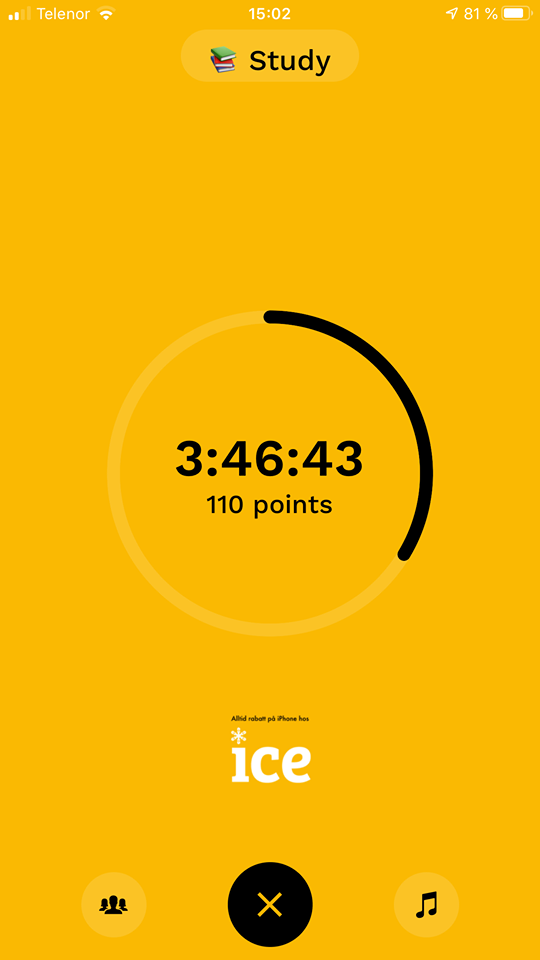
\includegraphics[width=.8\textwidth]{Images/ExistingGames/HoldApp.png}
              \captionof{figure}{Main timer screen in Hold}
              \label{fig:hold_timer}
            \end{minipage}
            \begin{minipage}{.5\textwidth}
              \centering
              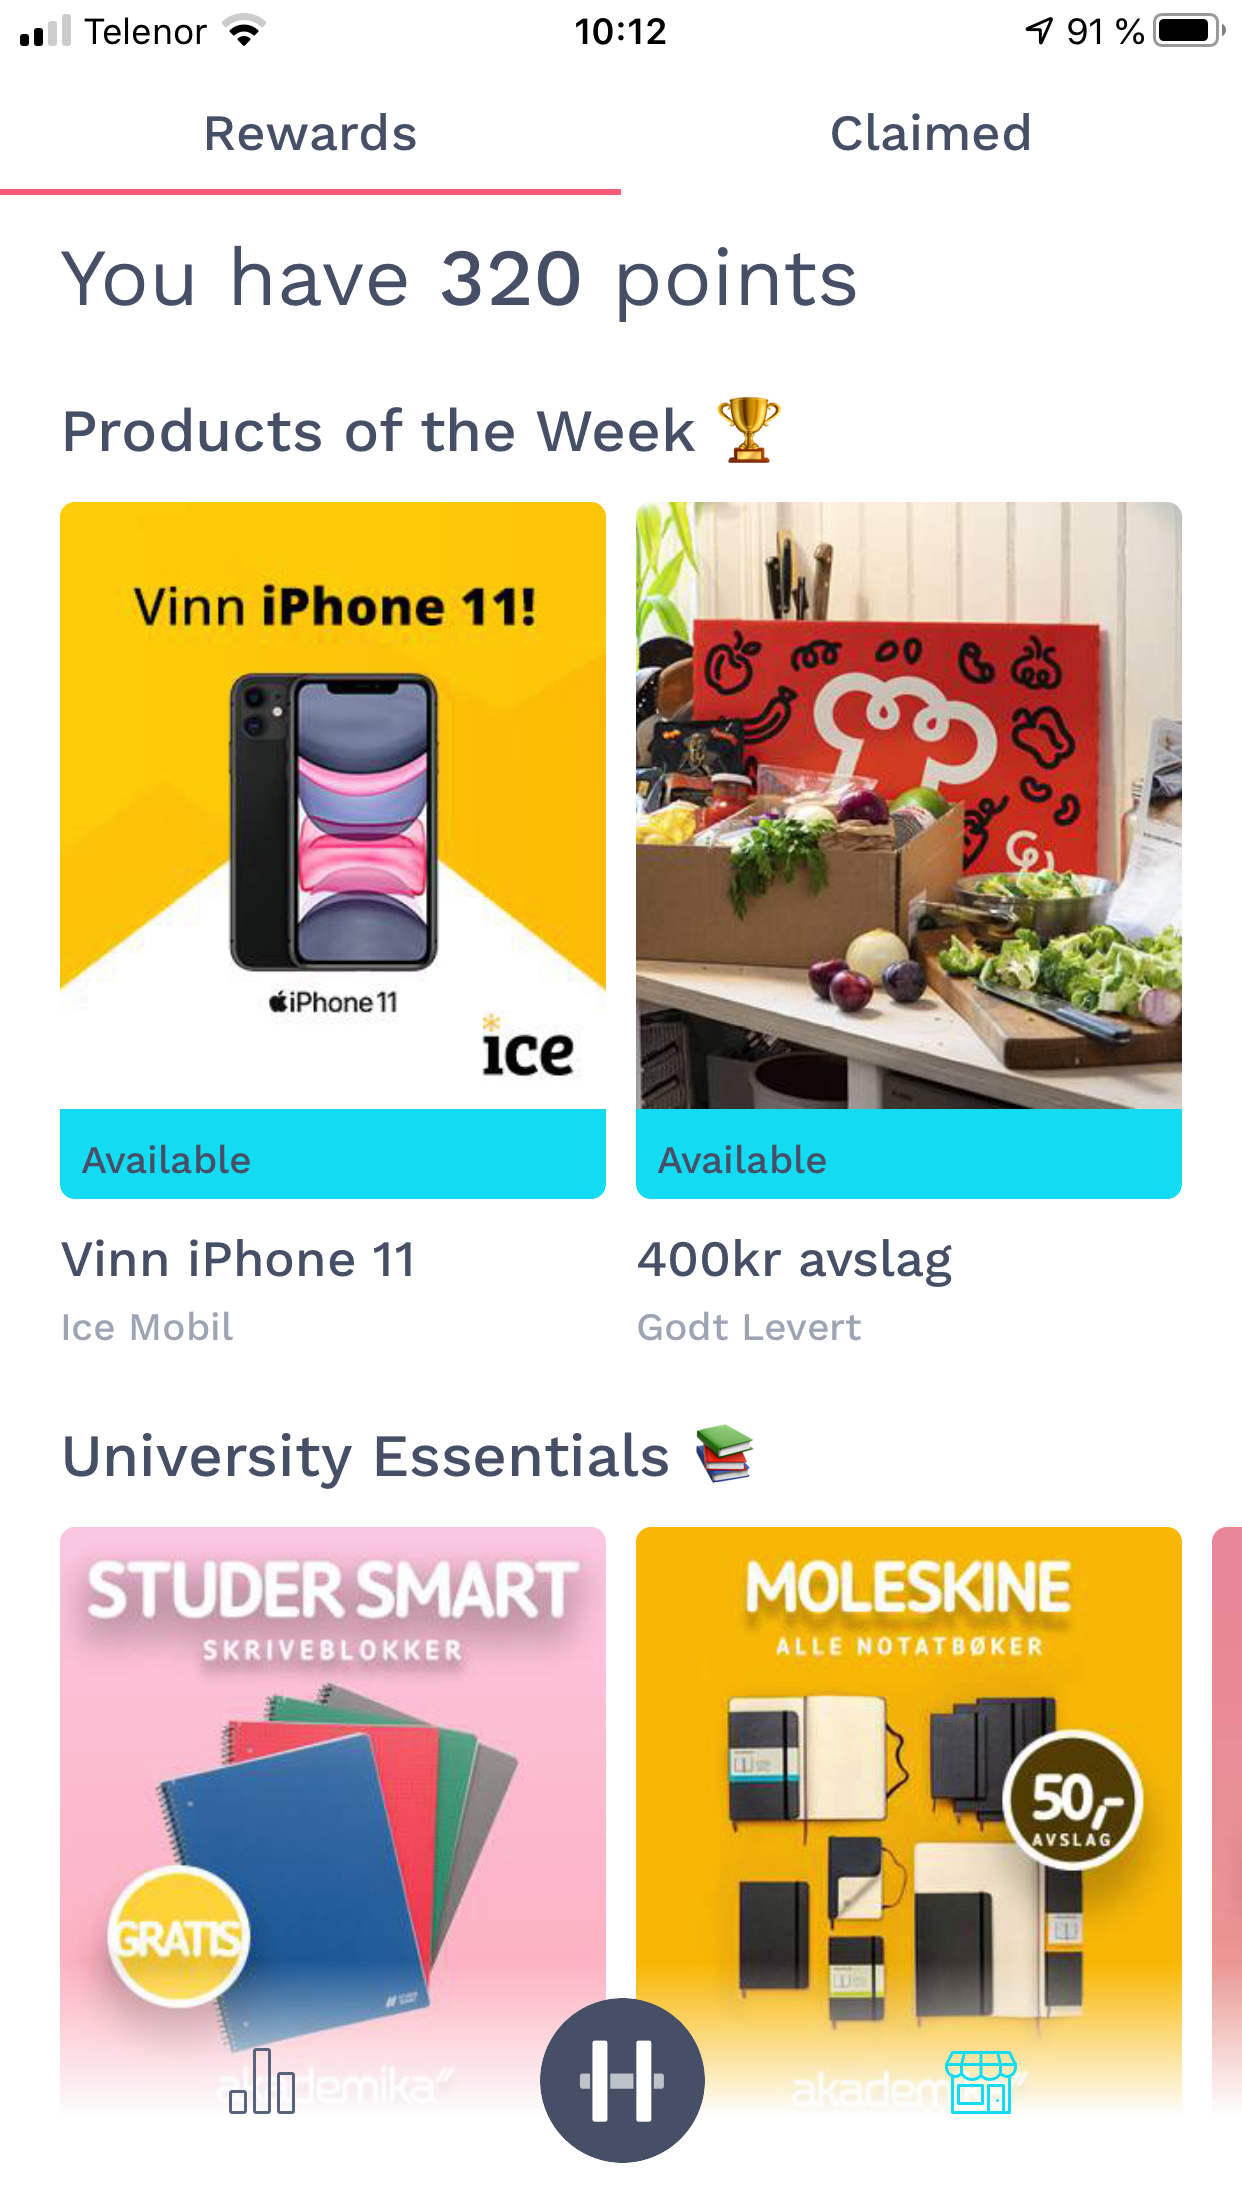
\includegraphics[width=.8\textwidth]{Images/ExistingGames/HoldAppRewards.png}
              \captionof{figure}{Choices of rewards in Hold}
              \label{fig:hold_reward}
            \end{minipage}
        \end{figure}

    \subsection{Mario Kart Live}
    Mario Kart Live is a newly developed augmented reality concept from Nintendo (released 16th October 2020). The game is based around the classic Mario Kart game, but with a rather unique twist: the inclusion of a specially designed RC kart that follows the user’s maneuvers in-game. A live video feed from the racing kart is relayed to the user’s Switch, mapping the virtual track to the user’s home \citep{velazco_race_2020}. The game can be played both individually (against AIs) or as a multiplayer game with more than one kart \citep{hashimoto_mario_2020}.
    
    The game is a typical example of how an alternative game can bring something new to an already familiar game concept, by using alternative input and output sources. Below is a screenshot from the game where you can see the karts racing a user’s home and how the game is presented to the player.
    \begin{figure}[H]
        \centering
        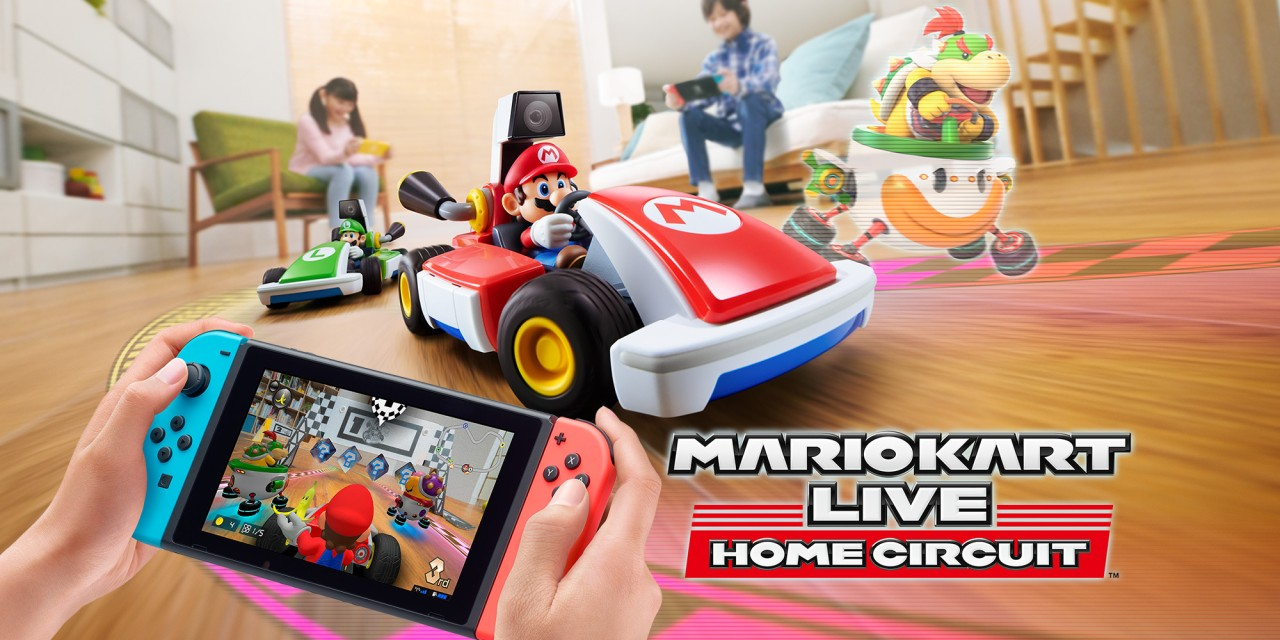
\includegraphics[width=0.8\textwidth]{Images/ExistingGames/MarioKartLive.jpeg}
        \caption{Mario Kart Live poster showing illustrated gameplay}
        \label{fig:mario_kart_live}
    \end{figure}

    \subsection{Pokemon Go}
    Pokémon Go is an alternative game published and developed by Niantic for iOS and Android. The game was launched in 2016 and quickly became one of the most popular mobile games of all time \citep{grubb_pokemon_2016}. The concept is an extension of the classic Pokémon game found on multiple of Nintendo's handheld devices. 

    \begin{figure}[H]
        \begin{minipage}{.5\textwidth}
          \centering
          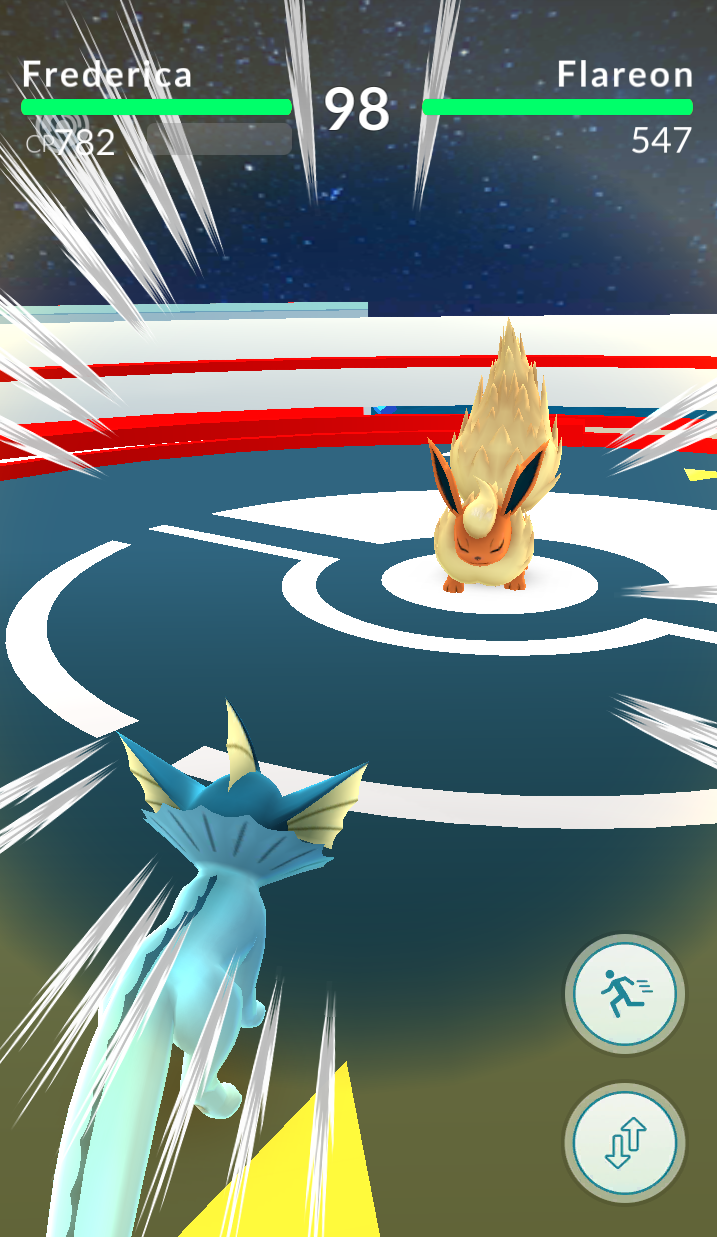
\includegraphics[width=.8\textwidth]{Images/ExistingGames/PokemonGoBattle.png}
          \captionof{figure}{Screenshot of battle in Pokemon Go}
          \label{fig:pokemon_go_battle}
        \end{minipage}
        \begin{minipage}{.5\textwidth}
          \centering
          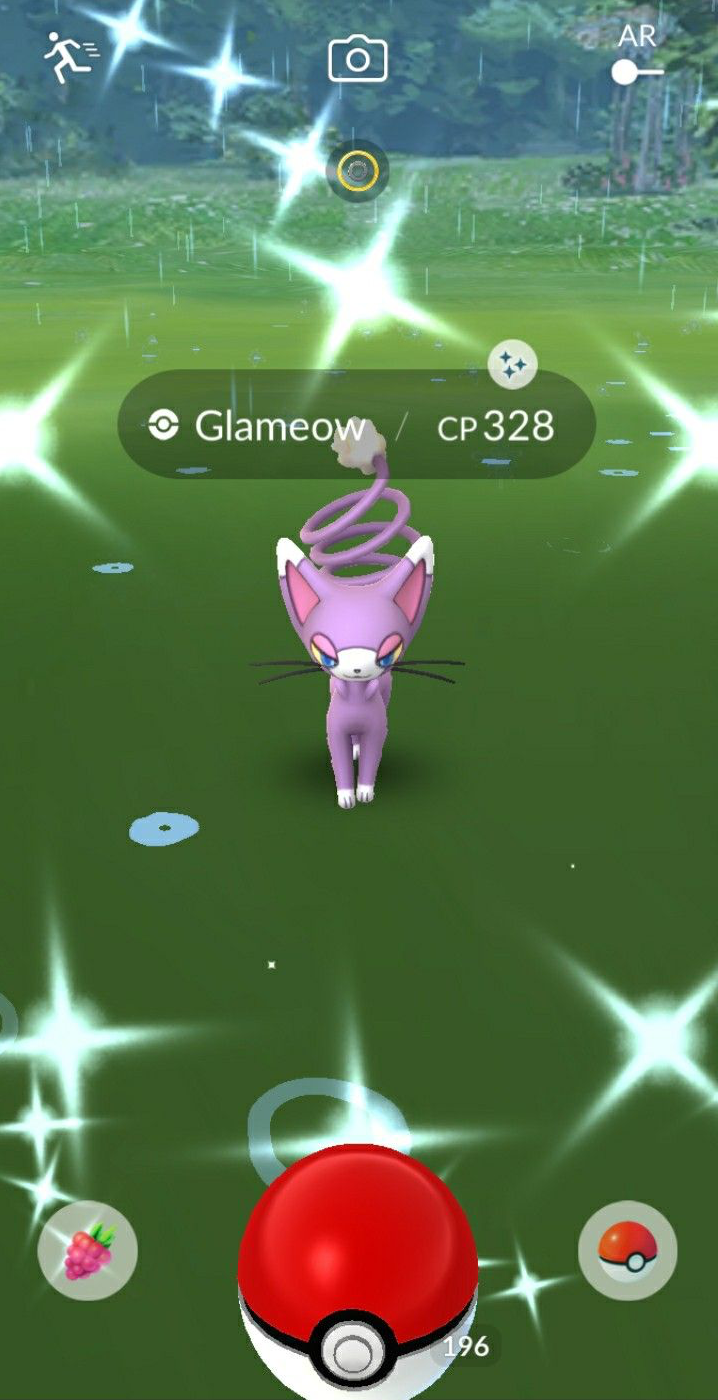
\includegraphics[width=.8\textwidth]{Images/ExistingGames/PokemonGoCatch.png}
          \captionof{figure}{Typical gameplay screenshot Pokemon Go}
          \label{fig:pokemon_go_catch}
        \end{minipage}
    \end{figure}

    The game concept is similar to the previous Pokémon games but utilizes AR and location determination (GPS) for the player to find and catch Pokémons. Meaning the player needs to move around in the real world to play the game. Battles between Pokémons (to increase combat points and get prices) can happen at specific places known as Pokémon Gyms. These spots correspond to real-world points of interest (POI) such as parks and tourist attractions \citep{bastow_pokestops_2016}. There are also additional important POI in the game, e.g. PokéStops and Nests. Figure \ref{fig:pokemon_go_battle} is an in-game screenshot where you can see a typical Pokémon battle, while figure \ref{fig:pokemon_go_catch} shows a screenshot of gameplay while catching a Pokémon.
    
    The game is clearly an alternative game as it explores uncommon input and output sources such as camera, GPS, and AR. Pokémon Go is a good example of how alternative games can be very successful. 
    
    \subsection{Just Dance Now}
        \begin{figure}[H]
            \begin{minipage}{.5\textwidth}
              \centering
              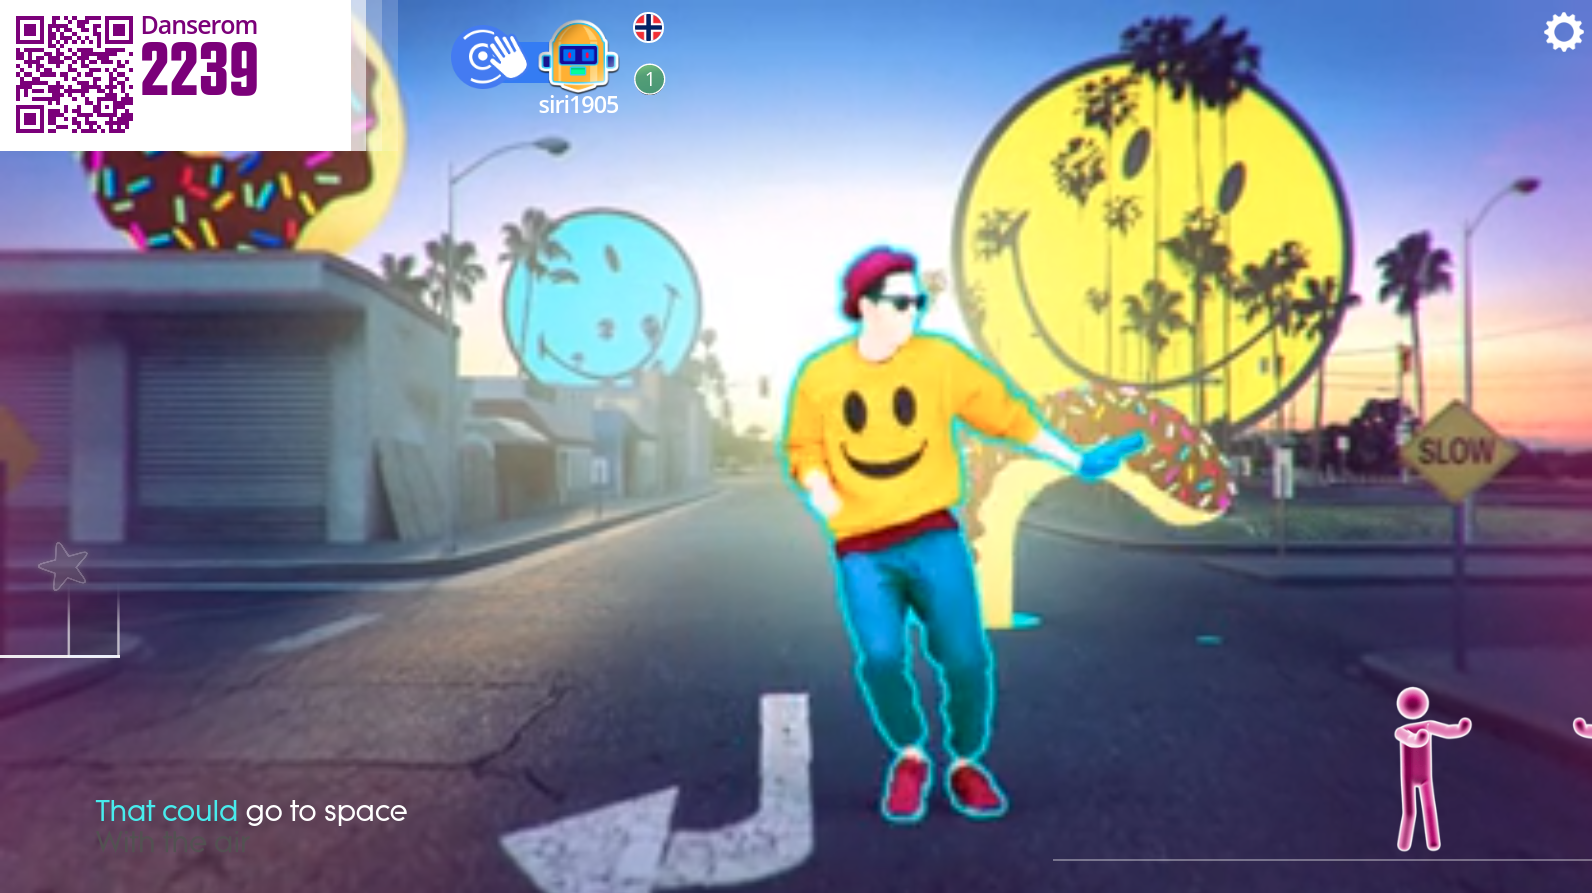
\includegraphics[width=.8\textwidth]{Images/ExistingGames/JustDanceNow_Pc.png}
              \captionof{figure}{Just Dance Now screenshot from PC}
              \label{fig:JustDanceNow_Pc}
            \end{minipage}
            \begin{minipage}{.5\textwidth}
              \centering
              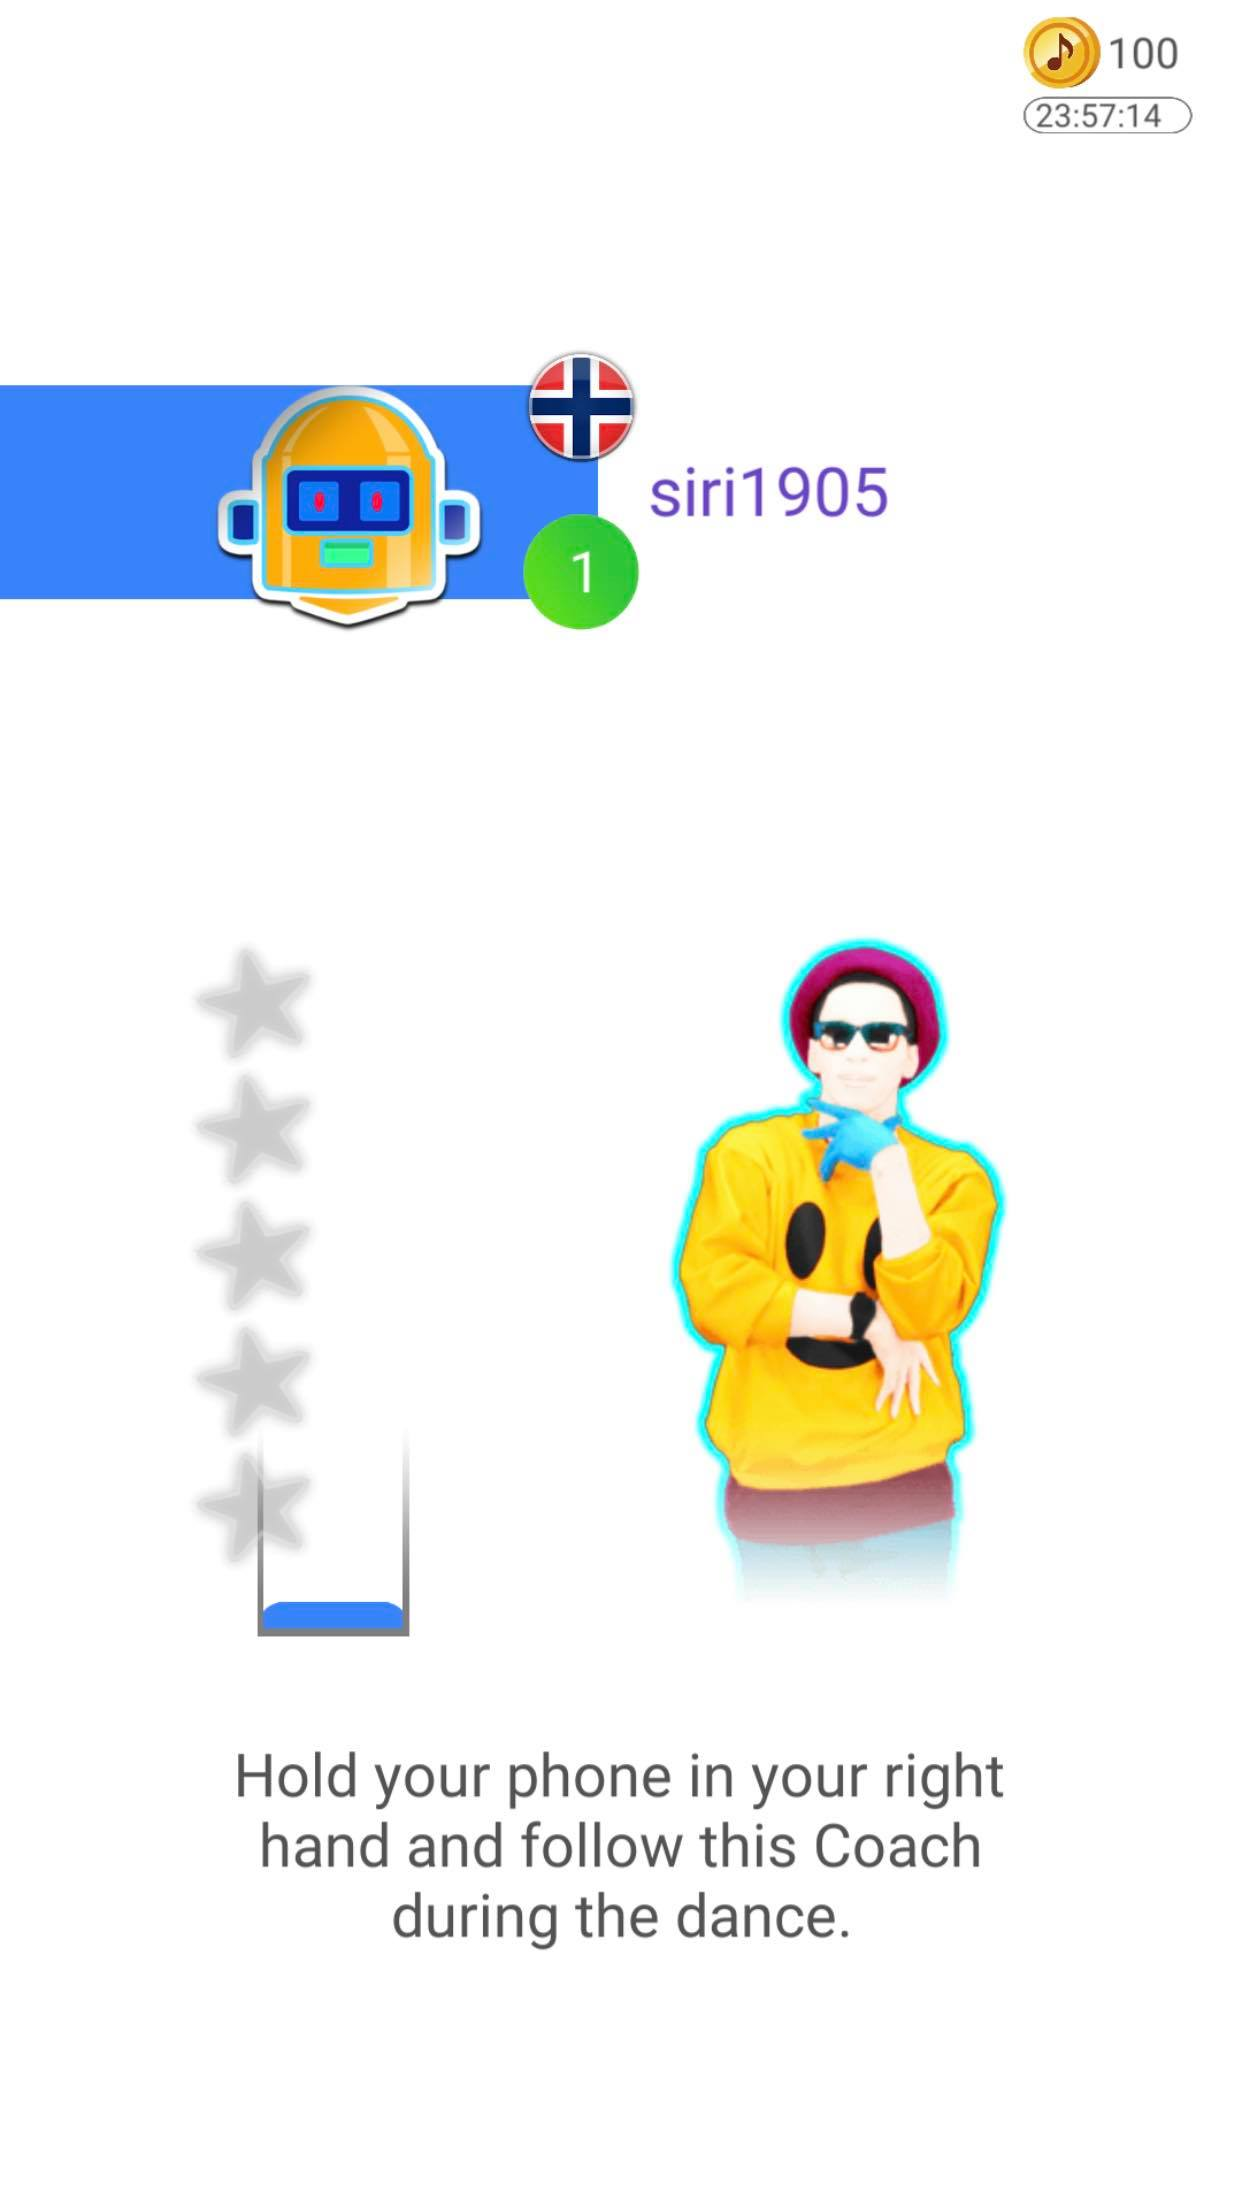
\includegraphics[width=.8\textwidth]{Images/ExistingGames/JustDanceNow_Mobile.jpg}
              \captionof{figure}{Just Dance Now screenshot from Mobile}
              \label{fig:JustDanceNow_Mobile}
            \end{minipage}
        \end{figure}
        
        \subsection{Guitar Hero}
        Guitar Hero is a series of games originally developed for PlayStation 2 in 2005. The game series later expanded to multiple other game platforms, including Xbox 360 and Nintendo Wii. The game concept is based on simulation and gamification of playing guitar, using a custom-developed guitar controller (see figure \ref{fig:guitar_hero_controller}). The player tries to match the in-game “notes” with buttons on the guitar controller, resulting in a score that is coherent with the number of notes hit. Songs available to choose from vary between different games, but generally, they belong to the genre of rock \cite{noauthor_guitar_2020}. Figure \ref{fig:guitar_hero_screenshot} shows a screenshot example from playing the game in single-player mode. 
        
        \begin{figure}[H]
            \begin{minipage}{.5\textwidth}
                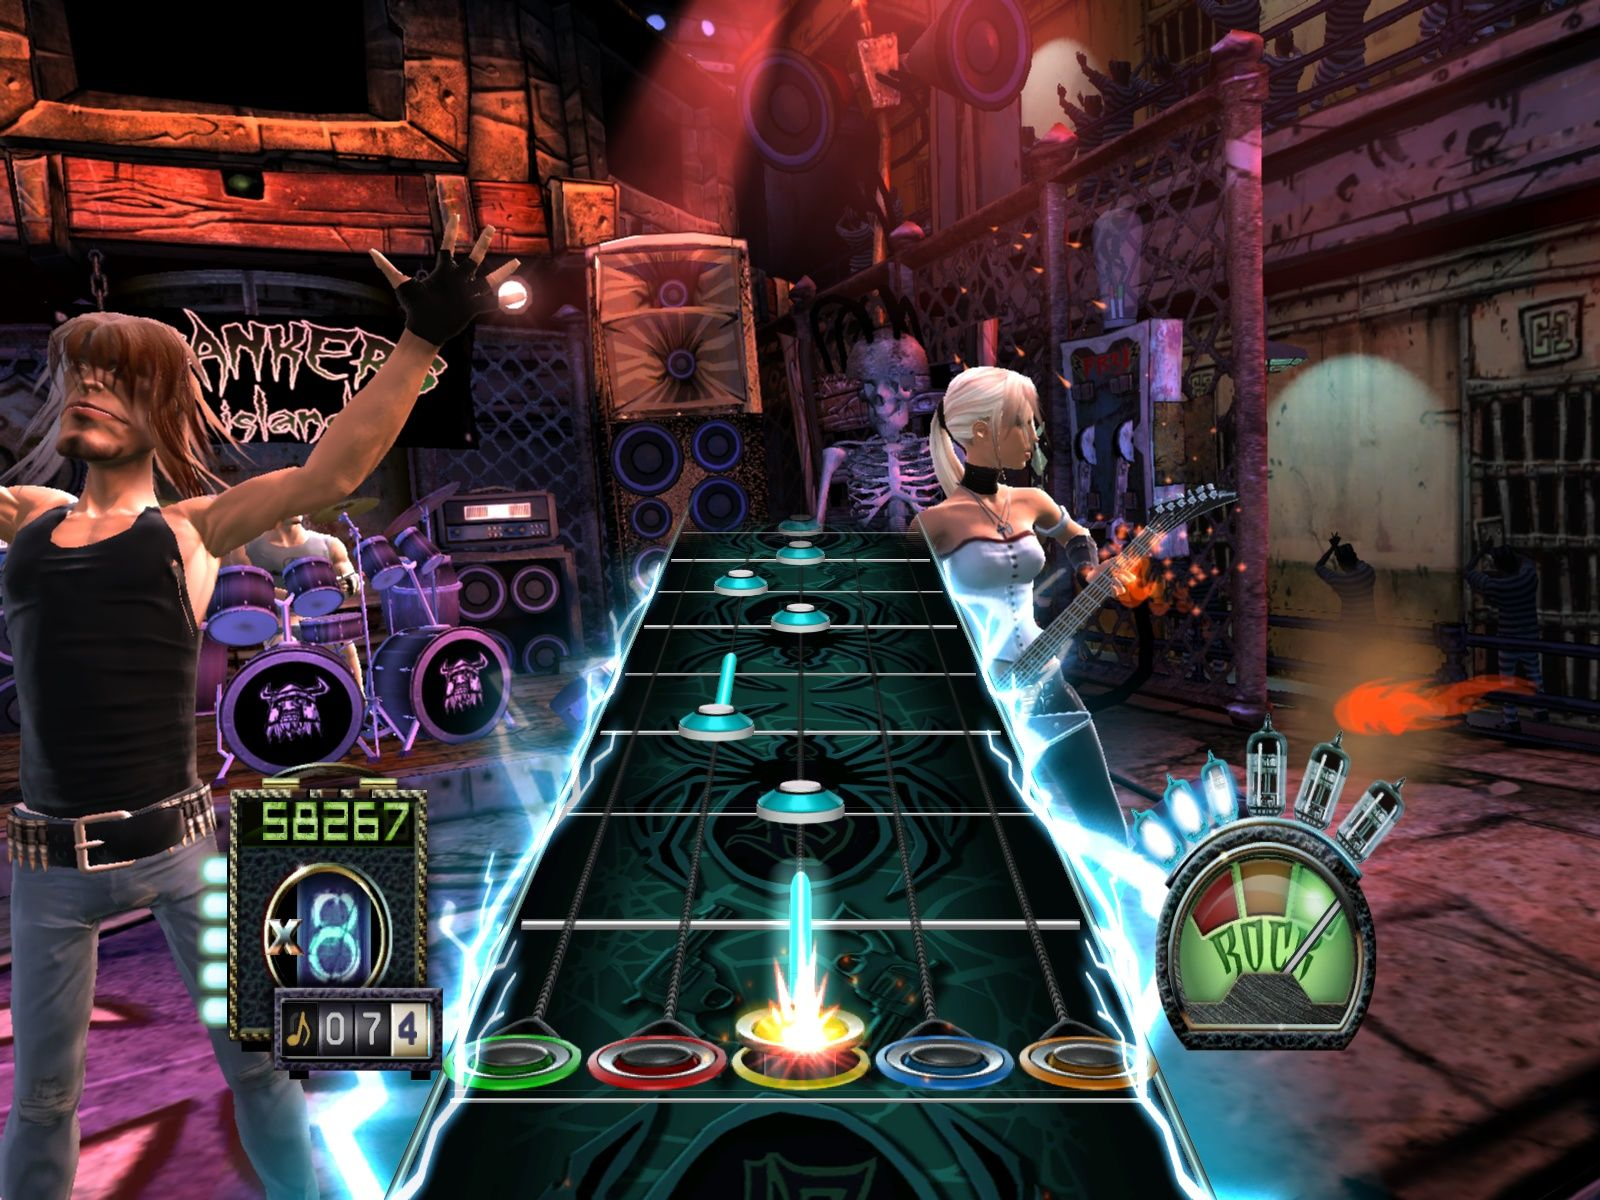
\includegraphics[width=0.8\textwidth]{Images/ExistingGames/GuitarHeroScreenshot.jpg}
                \caption{Screenshot from Guitar Hero Gameplay}
                \label{fig:guitar_hero_screenshot}
            \end{minipage}
            \begin{minipage}{.5\textwidth}
                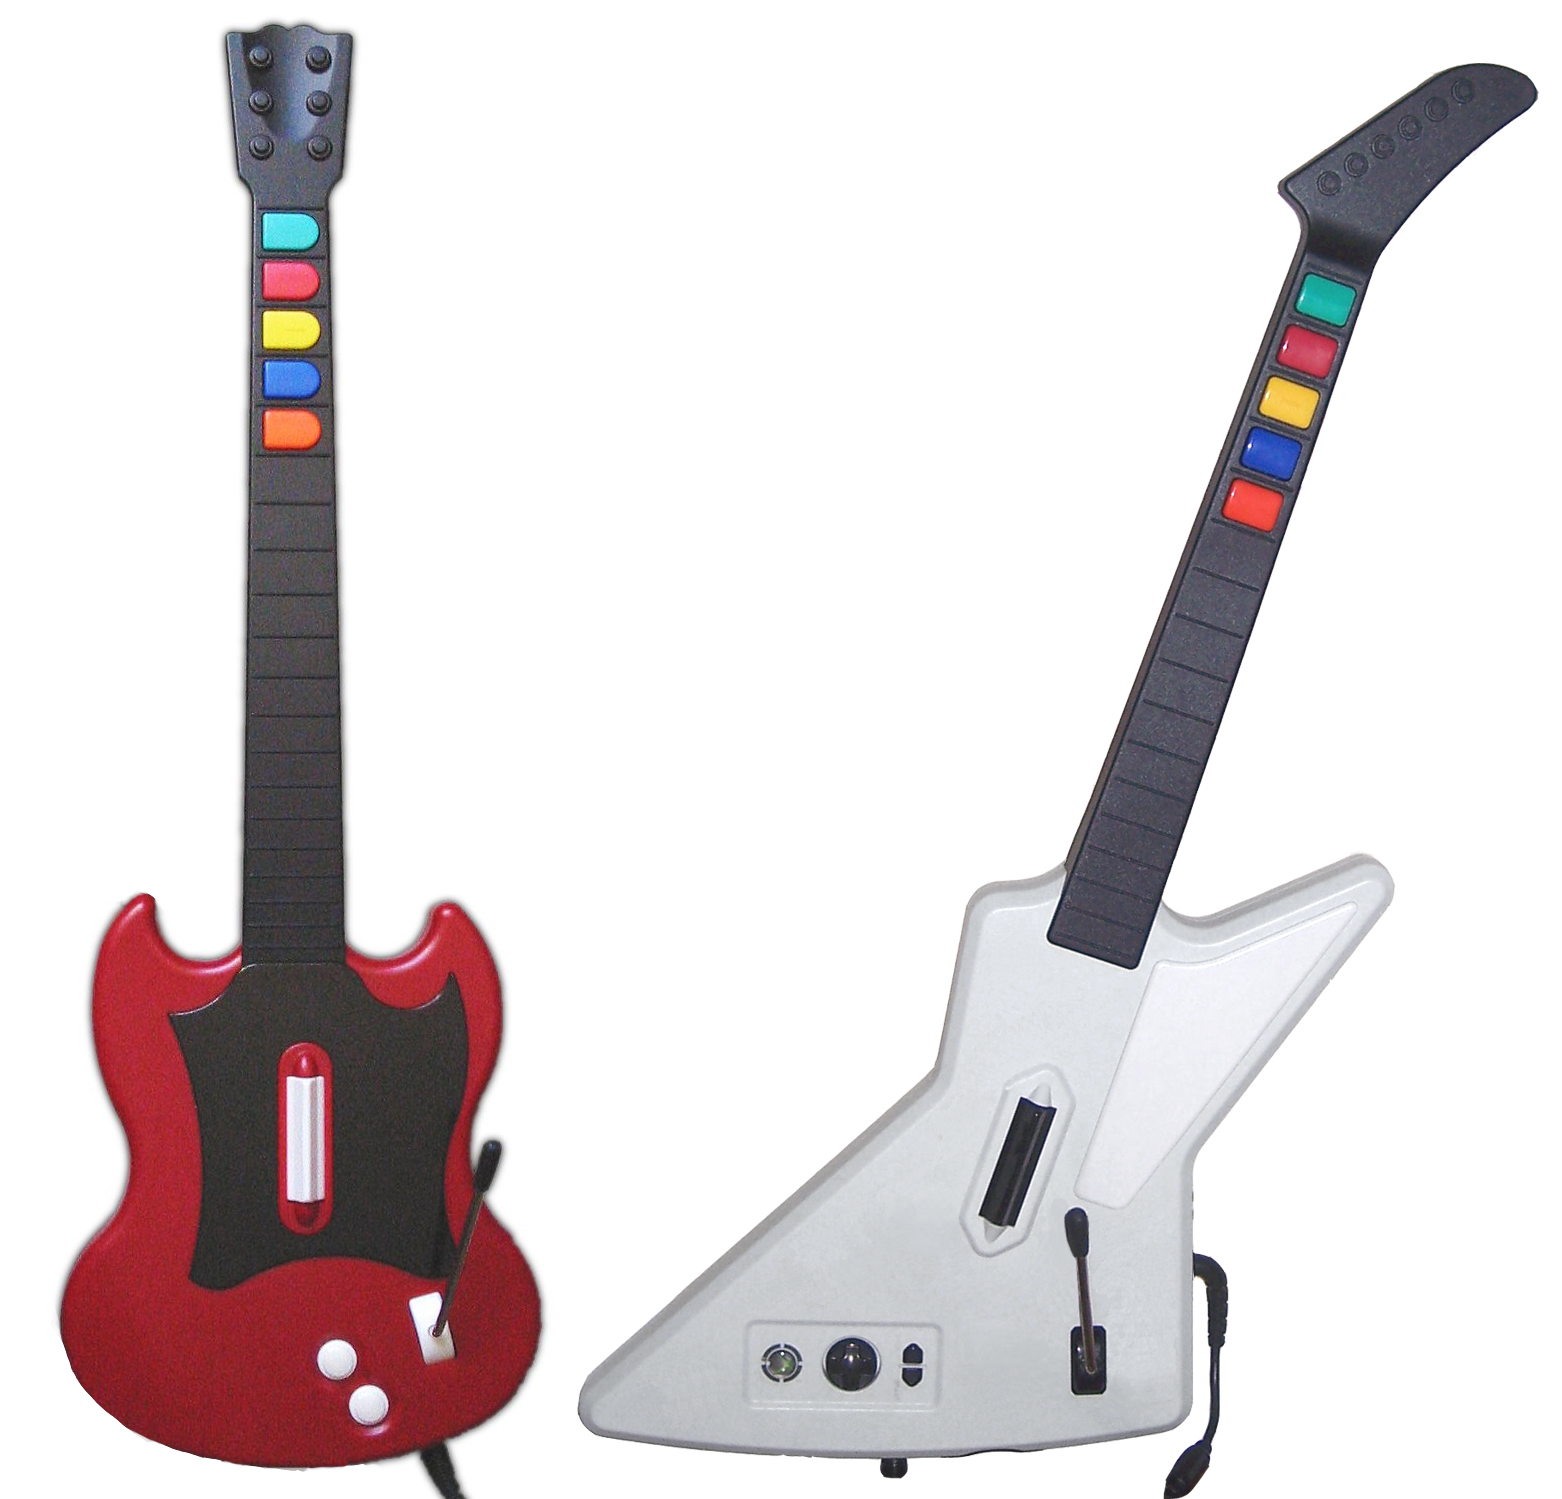
\includegraphics[width=0.8\textwidth]{Images/ExistingGames/GuitarHeroController.jpg}
                \caption{Example of Guitar Hero controllers}
                \label{fig:guitar_hero_controller}
            \end{minipage}
        \end{figure}
        
        One of the categories of alternative game characteristics is the input. A game using alternative input sources can be classified as an Alternative Game. Guitar Hero is a typical example of such a game because it depends on a custom-designed controller for playing the game.
        
        \subsection{Wii Fit}
        
        Wii Fit is an exergame(exercise-game) by Nintendo that launched in 2007 \citep{imdb_wii_2020}. The game is only available on Nintendo Wii and requires an additional controller in addition to the regular Wii controller. Wii Fit is a collection of minigames that combine the two domains of health and entertainment. The game has four main exercise categories to choose from; strength training, aerobics, yoga, and balance \citep{ign_wii_2008}. Each category has multiple minigames that are made to improve the player’s physical health in that specific category. 

        The additional controller is called the Wii Balance Board \citep{ign_wii_2008} and is one of the categories that makes the game alternative. The board’s purpose is to track the user's movement and translate that to the user’s in-game avatar. The idea behind the board was drawn from the bathroom weight, and it consists of four weight sensors; one in each corner. The controller connects to the console through bluetooth, where it calculates the user's movement in real-time \citep{jacquot_how_2010}. Based on the user’s movement, the game gives feedback on how the exercise is going. 
        
        In addition to the alternative input, the game is also a gamification of exercise. The game’s concept is to motivate players to get in shape from the comfort of their own home. The game focuses on providing a wide set of games that are engaging for the entire family. The game tracks all user’s progress and lets them compare themselves with other players. 

        
        \begin{figure}[H]
            \begin{minipage}{.5\textwidth}
                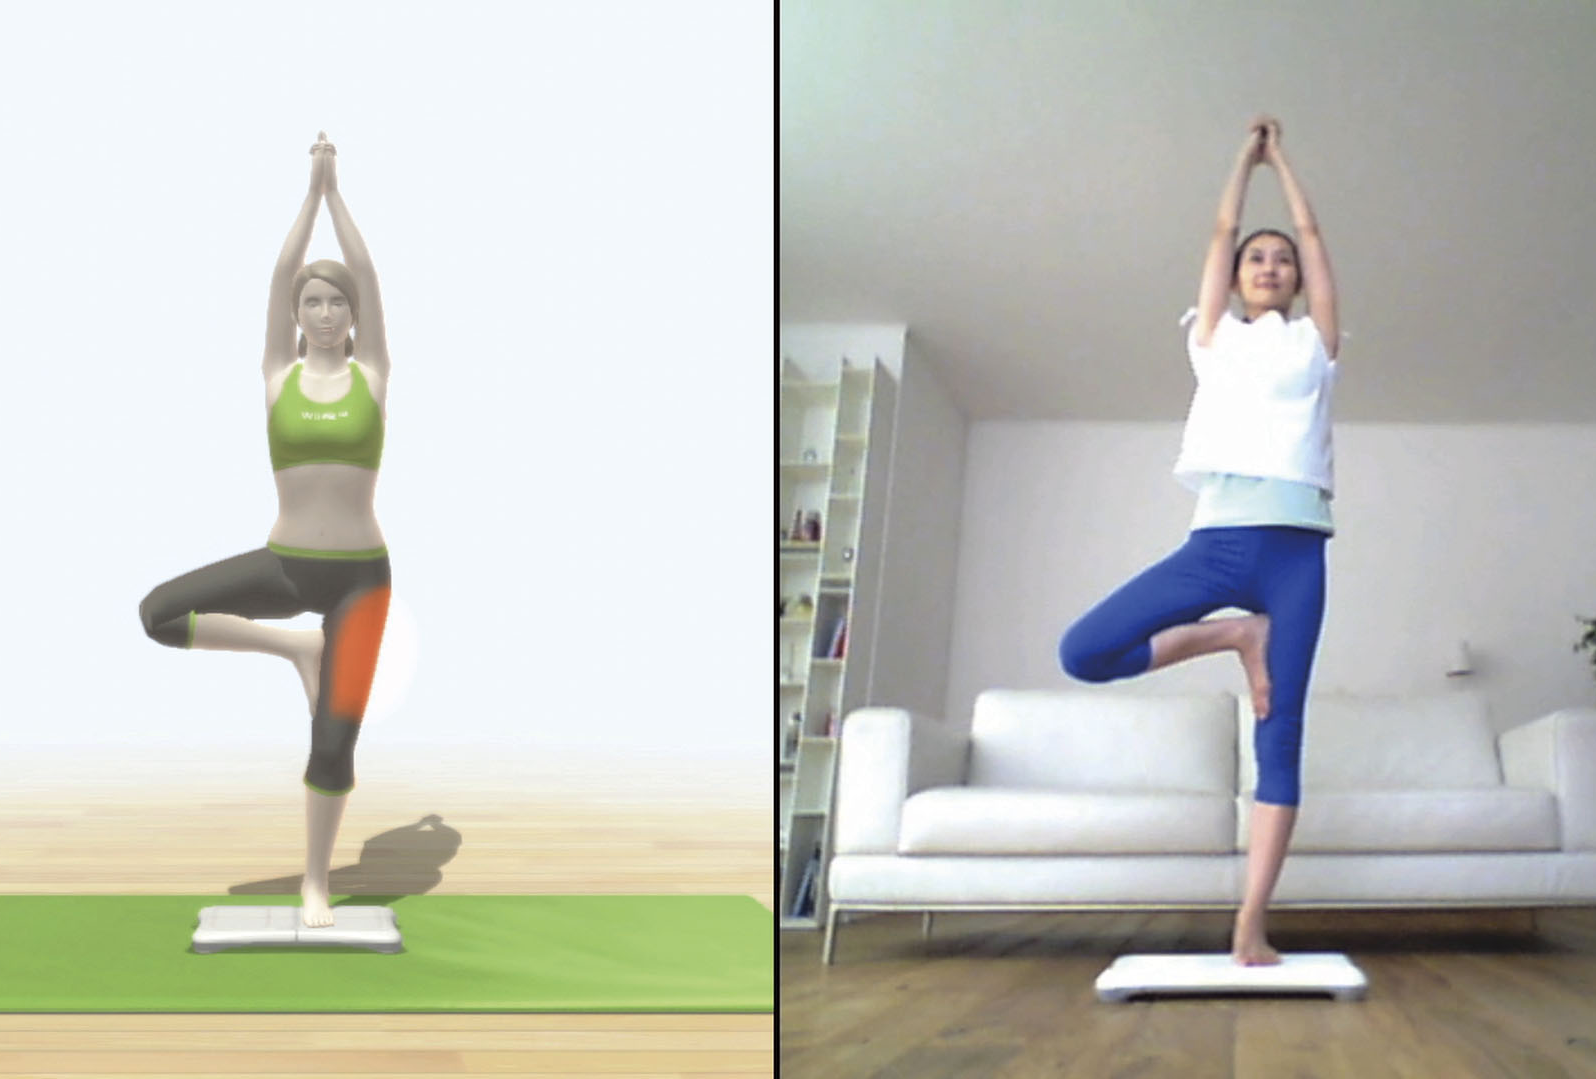
\includegraphics[width=0.8\textwidth]{Images/ExistingGames/WiiFit_Pose.png}
                \caption{Example of yoga exercise beside in-game avatar.}
                \label{fig:wii_fit_pose}
            \end{minipage}
            \begin{minipage}{.5\textwidth}
                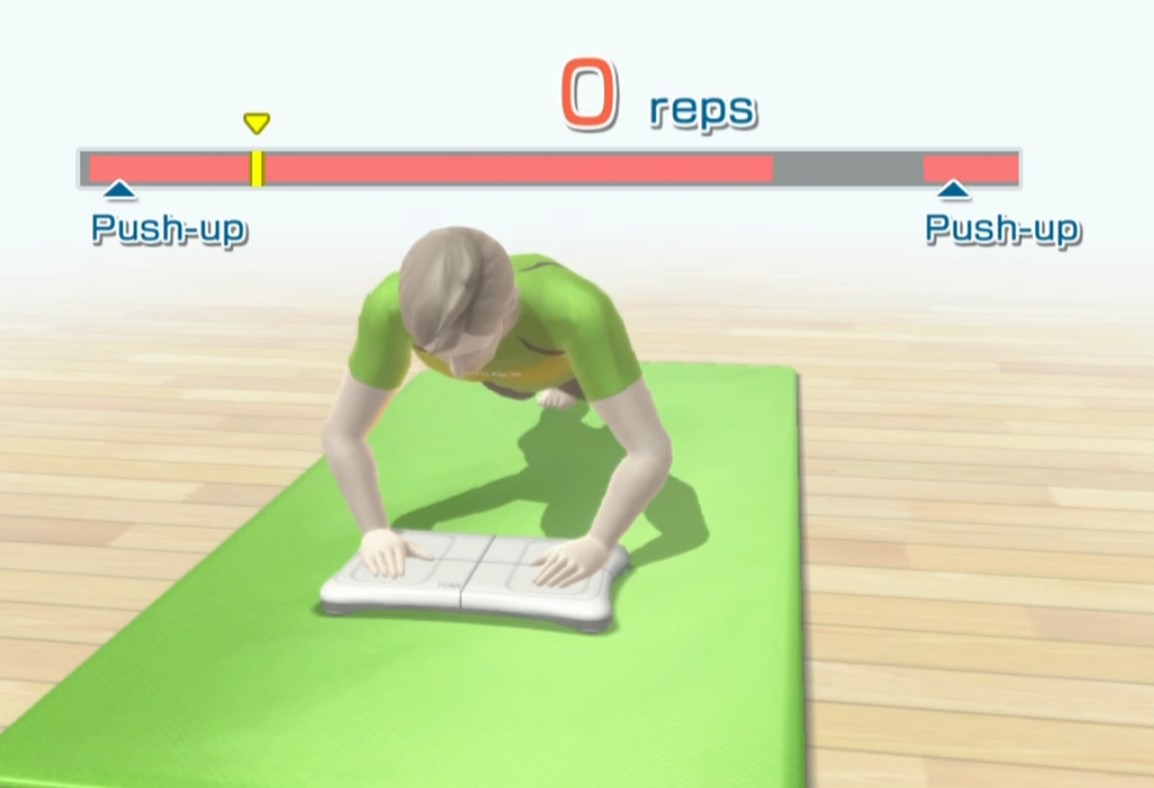
\includegraphics[width=0.8\textwidth]{Images/ExistingGames/WiiFit_Pushup.jpg}
                \caption{Screenshot of in-game avatar using the board to track push-ups. }
                \label{fig:wii_fit_pushup}
            \end{minipage}
        \end{figure}
    
    \subsection{Comparison}

\section{Technology review}

\section{Design an enjoyable game}
    \subsection{Gameflow}
        \citep{malone_what_1980, sweetser_gameflow_2005}
        \subsubsection{Concentration}
        \subsubsection{Challenge}
        \subsubsection{Skills}
        \subsubsection{Control}
        \subsubsection{Clear goals}
        \subsubsection{Feedback}
        \subsubsection{Immersion}
        \subsubsection{Social interaction}
    \subsection{What makes things fun to learn?}
        \subsubsection{Challenge}
        \subsubsection{Fantasy}
        \subsubsection{Curiosity}

\biblio % Needed for referencing to working when compiling individual subfiles - Do not remove
\end{document}